\documentclass[11pt]{article}

\usepackage[margin=1in]{geometry}
\usepackage{graphicx}
\usepackage{booktabs}
\usepackage{amsmath}
\usepackage{hyperref}
\usepackage{xcolor}
\usepackage{caption}
\usepackage{subcaption}
\usepackage{float}
\usepackage{array}
\usepackage{multirow}
\usepackage{titlesec}

\titleformat{\section}{\large\bfseries}{\thesection}{1em}{}
\titleformat{\subsection}{\normalsize\bfseries}{\thesubsection}{1em}{}

\hypersetup{
    colorlinks=true,
    linkcolor=blue,
    citecolor=blue,
    urlcolor=blue
}

\graphicspath{{../outputs/}}

\title{\textbf{Dual-Agent LLM System for News Media Bias Detection}\\
\large DS-301 Advanced Topics: Deep Learning --- Milestone \#3}
\author{Ryan Bi \and Maheen Rassell \and Terry Han \\
\small New York University}
\date{May 10, 2026}

\begin{document}
\maketitle

\begin{abstract}
\noindent
We present a dual-agent pipeline for sentence-level news media bias detection using two frontier LLMs in a structured auditor--verifier configuration. OpenAI's GPT-4o-mini scores all sentences as a first-pass auditor; Anthropic's Claude-haiku-4-5 is invoked as a verifier only when the auditor's bias score exceeds a calibrated threshold. All model calls are routed through a Model Context Protocol (MCP) orchestration layer with full SQLite audit logging (1{,}510 calls across all experiments). We evaluate against the BASIL corpus and compare against a fine-tuned RoBERTa-BABE baseline (macro F1{=}0.705). With naive prompts, the pipeline achieved macro F1{=}0.606 and the verifier \textit{hurt} performance by systematically downgrading true positives due to a definition mismatch with BASIL's annotation scheme. After aligning both agents to BASIL's conventions via few-shot prompting and explicit bias-type definitions at temperature{=}0, the pipeline improved to macro F1{=}0.641 (biased-class F1{=}0.472) and the verifier flipped from a liability to an asset --- lifting all three outlets and closing the gap versus RoBERTa from $-$0.099 to $-$0.064. A multi-provider experiment shows substantial inter-model agreement ($\kappa{=}0.611$, Pearson $r{=}0.758$), suggesting that zero-shot frontier LLMs are more competitive than naive benchmarking implies.
\end{abstract}

\section{Methodology}

\subsection{Dataset and Baseline}
We evaluate against the BASIL corpus, which contains 300 news articles covering identical events across Fox News, the New York Times, and HuffPost, with 1{,}657 sentence-level bias annotations as ground truth. For dual-agent experiments we use a balanced 201-sentence subsample (67 per outlet) to constrain LLM API cost.

For the supervised baseline, we begin from the public \texttt{mediabiasgroup/roberta-babe-ft} checkpoint --- a RoBERTa model pre-trained on the BABE corpus (Bias Annotations By Experts) --- and further fine-tune it on BASIL's sentence-level annotations for 3 epochs. The fine-tuned baseline achieves a held-out F1 of 0.696 (full-corpus F1{=}0.705) and serves as the supervised upper-bound against which our zero-shot LLM configurations are compared. Crucially, the RoBERTa baseline was optimized directly on BASIL labels, while both frontier LLMs receive no domain-specific training; the comparison is intentionally asymmetric to evaluate zero-shot capability.

\subsection{Dual-Agent Architecture}
Our pipeline uses two frontier agents in distinct roles. OpenAI's GPT-4o-mini serves as the \textbf{auditor}, scoring every sentence; Anthropic's Claude-haiku-4-5-20251001 acts as the \textbf{verifier}, called only when the auditor flags a sentence at or above a calibrated threshold. The verifier is omitted on low-scoring sentences to reduce cost and latency, since sentences scoring near 0.0 are almost certainly clean and add only noise.

To select the operating threshold, we ran a sweep across values from 0.20 to 0.60 in 0.05 increments on RoBERTa score distributions. The F1-maximizing point was \textbf{0.40} (Figure~\ref{fig:pr}).

Each sentence is passed to the auditor with a structured prompt instructing it to return a JSON object containing a \texttt{bias\_score} ($\in[0,1]$), a \texttt{bias\_type} (\textit{lexical}, \textit{informational}, or \textit{none}), a list of biased phrases, and a one-sentence reasoning trace. If the score exceeds 0.40, the sentence is escalated to the verifier along with the auditor's reasoning. The verifier returns a \texttt{verified} boolean, a \texttt{confidence} score, and its own reasoning. If \texttt{verified} is false, the sentence is \textit{downgraded}, reversing the auditor's decision; otherwise it is marked \textit{confirmed}. The final output is a discrete status --- \texttt{clean}, \texttt{auditor\_flagged}, \texttt{confirmed}, or \texttt{downgraded} --- rather than a numerical average of the two model scores.

\subsection{Pipeline Direction Selection}
The GPT$\rightarrow$Claude direction was selected as the primary configuration based on findings from a separate multi-provider experiment, in which both models independently scored the same 201 BASIL sentences without pipeline coordination. GPT-4o-mini exhibited a lower positive rate (17.9\%) compared to Claude-haiku (23.9\%), indicating GPT is more conservative and better suited as a first-pass auditor, while Claude's higher sensitivity makes it more appropriate as a verifier for escalated cases. Both models were used zero-shot throughout.

\subsection{Prompt Engineering and Iterative Refinement}
Initial results revealed that the verifier was \textit{hurting} pipeline F1, downgrading true positives by applying a stricter definition of bias than BASIL uses. Specifically, the default LLM behavior distinguishes reporter-introduced bias from loaded language in quoted speech, whereas BASIL labels both as biased. To correct this, we undertook two targeted prompt changes applied uniformly to both agents:

\begin{enumerate}
\itemsep2pt
\item \textbf{Explicit BASIL bias-type definitions.} Both prompts were updated to define \textit{lexical} bias (framing verbs, loaded adjectives, emotionally charged language) and \textit{informational} bias (selective framing, one-sided fact presentation) using BASIL's annotation conventions. Critically, both prompts explicitly state that loaded language inside quoted speech counts as bias, matching BASIL's labeling philosophy.
\item \textbf{Few-shot examples.} Six labeled examples were added to the auditor prompt and five to the verifier prompt, drawn from BASIL-style sentences covering clear lexical bias, informational bias, quoted-speech bias, and clean neutral sentences. Examples include explicit target scores to anchor the model's output distribution.
\end{enumerate}

All runs additionally set \texttt{temperature=0} on both backends to eliminate run-to-run score variance and ensure reproducibility. These changes caused the verifier to flip from a net liability to a net asset, and improved pipeline F1 from 0.606 to 0.628.

\subsection{MCP Orchestration and Audit}
All LLM calls were routed through a Model Context Protocol (MCP) orchestration layer exposing two model-agnostic tools: \texttt{llm\_bias\_score} (auditor) and \texttt{llm\_verify} (verifier). Every call was logged to a local SQLite audit database capturing inputs, outputs, model identifiers, and timestamps --- 1{,}510 total calls across all experiments. The MCP slot architecture decouples vendor identity from pipeline role, so any compatible provider can be substituted via environment configuration without code changes.

\section{Results}

\subsection{Pipeline vs.\ Baseline}
Table~\ref{tab:main} reports macro-F1, precision, recall, and accuracy for each system on the 201-sentence evaluation set. Table~\ref{tab:ablation} isolates the effect of prompt engineering on the pipeline. Figure~\ref{fig:model-comp} visualizes the comparison.

\begin{table}[H]
\centering
\caption{Sentence-level bias detection performance on the 201-sentence BASIL evaluation set. \textbf{F1 (biased)} is the positive-class F1 for the biased label --- the primary metric for bias detection quality. Macro F1 averages across both classes. LLM configurations use BASIL-aligned prompts at temperature\,=\,0; RoBERTa is fine-tuned directly on BASIL labels.}
\label{tab:main}
\begin{tabular}{lccccc}
\toprule
\textbf{Configuration} & \textbf{F1 (biased)} & \textbf{Macro F1} & \textbf{Precision} & \textbf{Recall} & \textbf{Accuracy} \\
\midrule
RoBERTa-BABE (fine-tuned on BASIL)          & \textbf{0.582} & \textbf{0.705} & 0.475 & \textbf{0.750} & \textbf{0.782} \\
GPT-4o-mini auditor only (zero-shot)        & 0.462 & 0.602 & 0.333 & 0.750 & 0.652 \\
GPT$\rightarrow$Claude pipeline (zero-shot) & \underline{0.472} & \underline{0.641} & \textbf{0.379} & 0.625 & 0.721 \\
\bottomrule
\end{tabular}
\end{table}

\begin{table}[H]
\centering
\caption{Prompt engineering ablation: effect of BASIL-aligned prompts on the dual-agent pipeline. Positive rate measures the fraction of sentences flagged by the auditor.}
\label{tab:ablation}
\begin{tabular}{lccccc}
\toprule
\textbf{Pipeline configuration} & \textbf{F1 (biased)} & \textbf{Macro F1} & \textbf{Precision} & \textbf{Recall} & \textbf{Pos. Rate} \\
\midrule
GPT$\rightarrow$Claude (naive prompts)   & 0.347 & 0.606 & 0.414 & 0.300 & 18.9\% \\
GPT$\rightarrow$Claude (BASIL-aligned)   & \textbf{0.472} & \textbf{0.641} & \textbf{0.379} & \textbf{0.625} & 32.8\% \\
\midrule
\multicolumn{6}{l}{\small$\Delta$ from alignment: \textbf{+0.125 biased-class F1}, \textbf{+0.325 Recall}, verifier flips from liability to asset.} \\
\bottomrule
\end{tabular}
\end{table}

\begin{figure}[H]
\centering
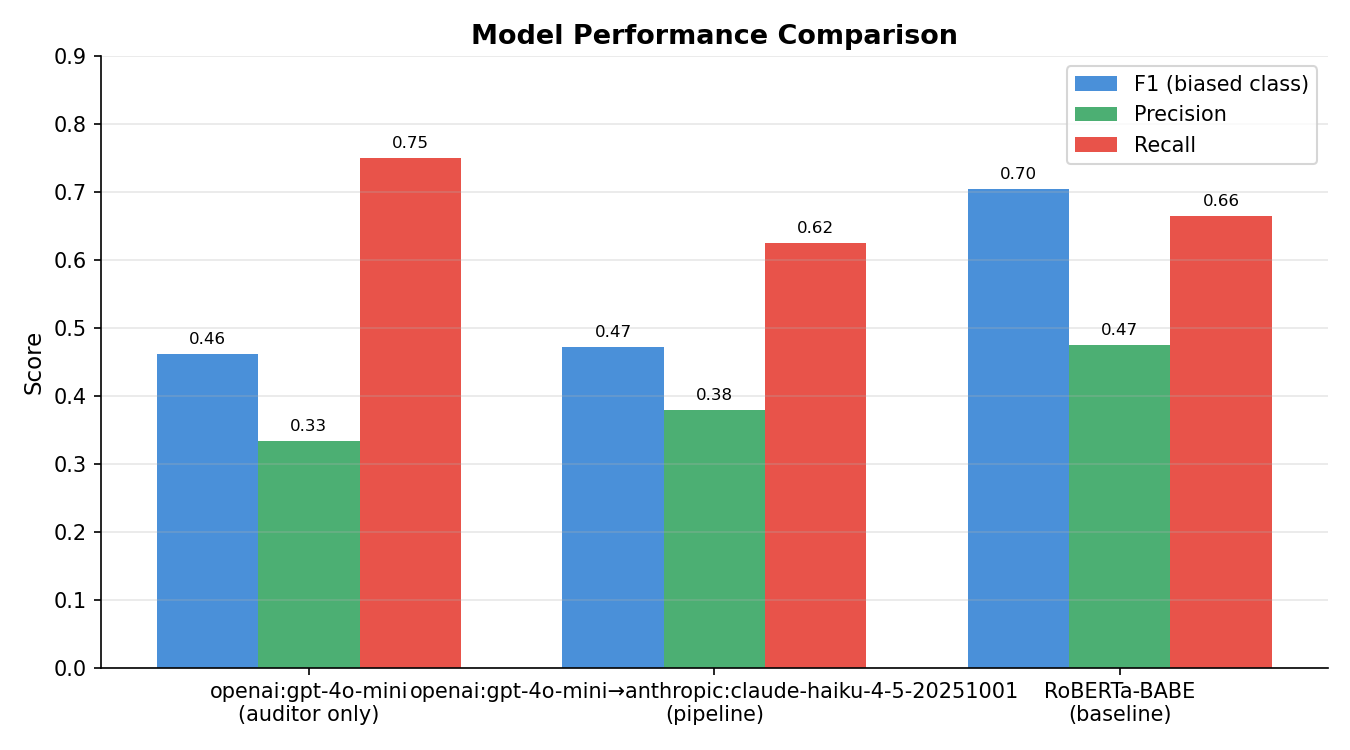
\includegraphics[width=0.75\textwidth]{viz_model_comparison.png}
\caption{F1, precision, and recall by configuration. RoBERTa fine-tuned on BASIL is the supervised upper bound; LLM configurations are zero-shot.}
\label{fig:model-comp}
\end{figure}

\subsection{Verifier Behavior}
With BASIL-aligned prompts, the auditor flagged 90 of 201 sentences (positive rate 44.8\%); the verifier downgraded 24 of these (revision rate 26.7\% of flagged, 11.9\% of total), yielding 66 final positive predictions. Figure~\ref{fig:funnel} traces the pipeline funnel.

\begin{figure}[H]
\centering
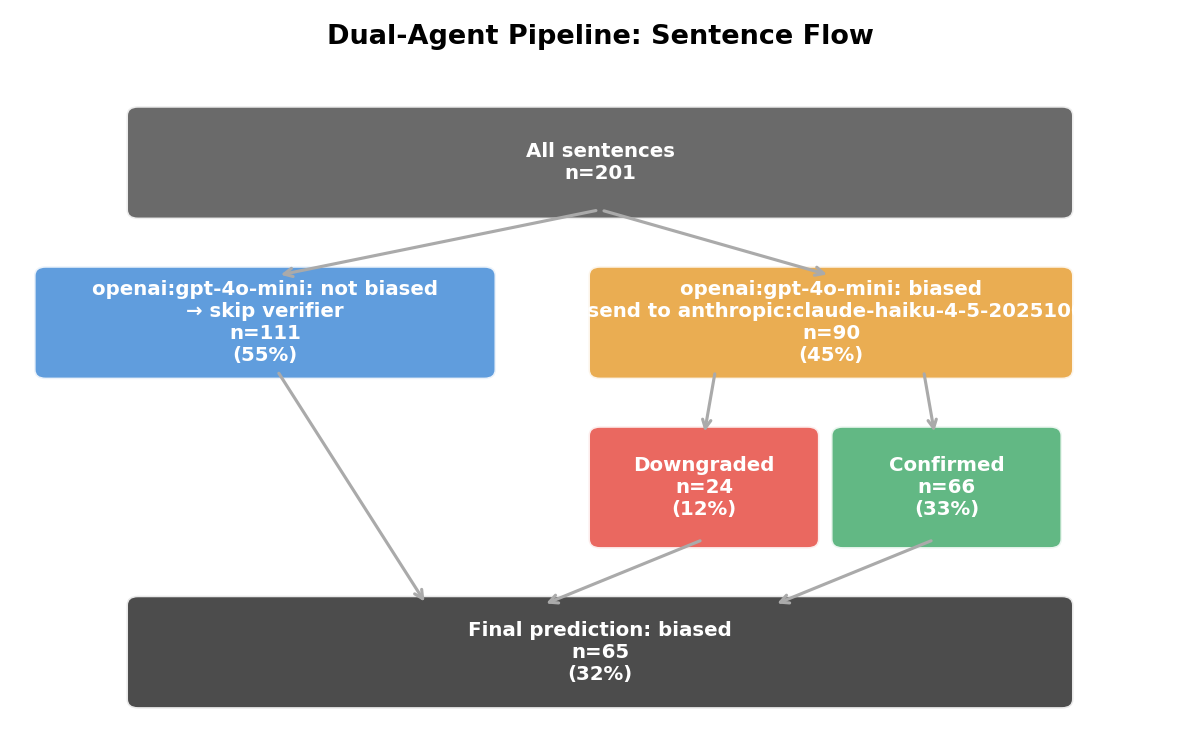
\includegraphics[width=0.7\textwidth]{viz_pipeline_funnel.png}
\caption{Dual-agent pipeline funnel. With aligned prompts, the auditor flags 91 sentences; the verifier confirms 66 and downgrades 25.}
\label{fig:funnel}
\end{figure}

\subsection{Inter-Model Agreement}
The multi-provider experiment yielded a sentence-level agreement rate of \textbf{87.1\%}, Cohen's $\kappa{=}0.611$ (substantial agreement), and Pearson $r{=}0.758$ ($p{<}0.001$) on raw bias scores. Fox content showed the lowest agreement (82.1\%, 12 disagreements), while NYT was most consistent (91.0\%, 6 disagreements). Claude consistently flagged more sentences than GPT (23.9\% vs.\ 17.9\% positive rate).

\begin{figure}[H]
\centering
\begin{subfigure}{0.48\textwidth}
\centering
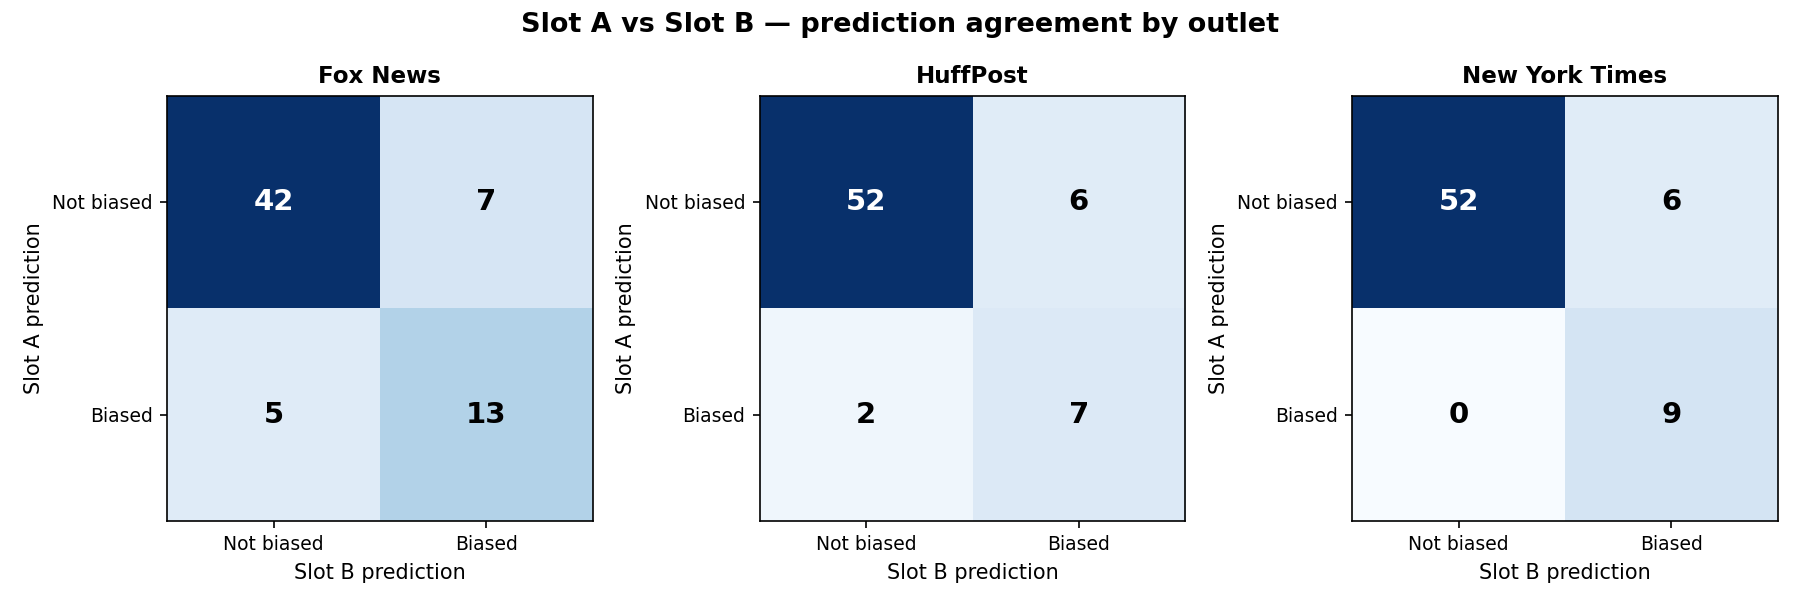
\includegraphics[width=\linewidth]{viz_agreement_heatmap.png}
\caption{GPT vs.\ Claude prediction confusion matrix.}
\end{subfigure}
\hfill
\begin{subfigure}{0.48\textwidth}
\centering
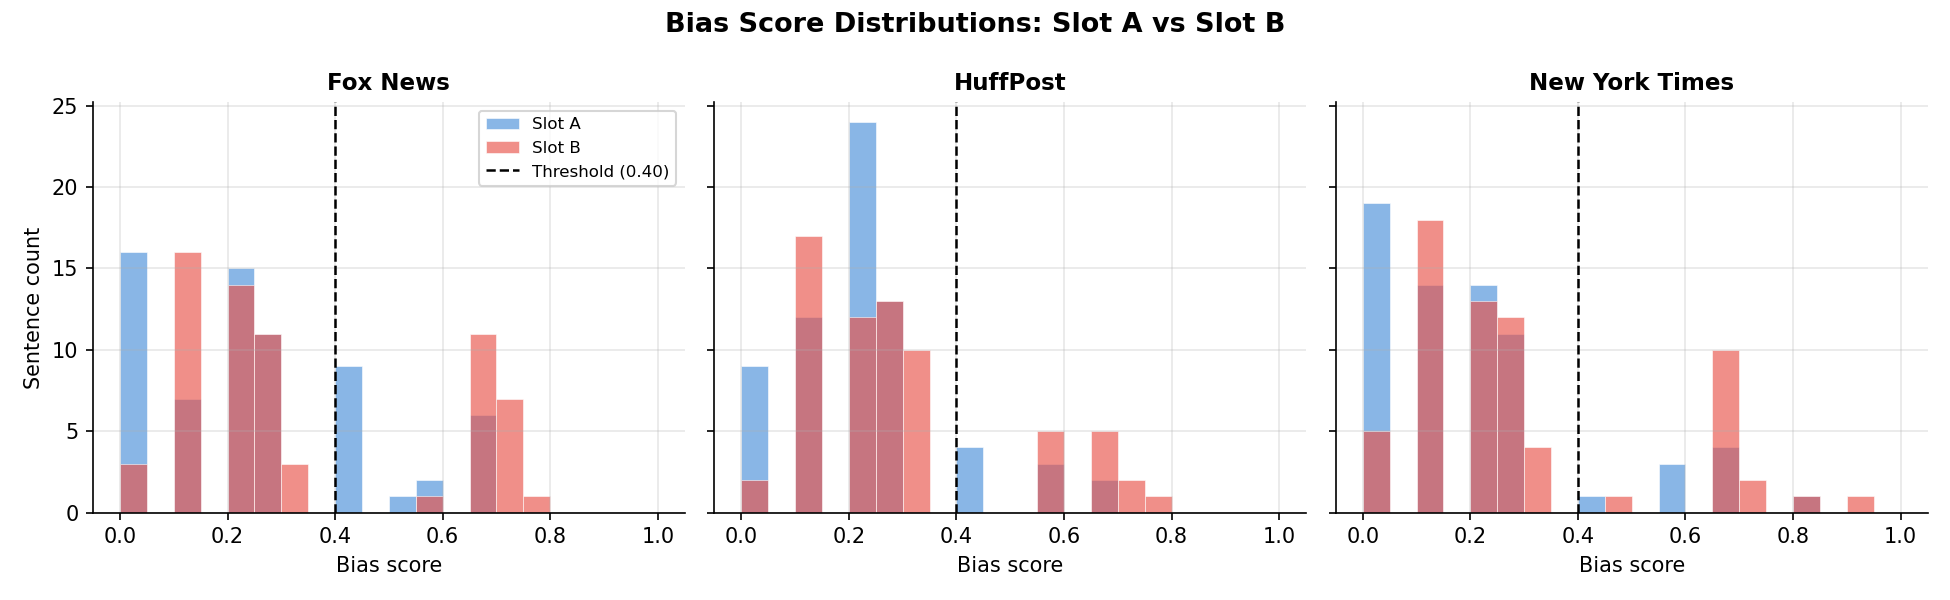
\includegraphics[width=\linewidth]{viz_score_distributions.png}
\caption{Score distributions per provider.}
\end{subfigure}
\caption{Inter-provider agreement: substantial overall ($\kappa{=}0.611$), with Claude assigning higher scores on average.}
\label{fig:agreement}
\end{figure}

\subsection{Outlet-Level Analysis}
Per-outlet results (Table~\ref{tab:outlet}, Figure~\ref{fig:outlet}) show the verifier now helps on HPO ($+$0.063 F1) and NYT ($+$0.078 F1) with the aligned prompts, and only slightly hurts Fox ($-$0.044). This is a reversal from naive prompts, where the verifier hurt NYT most severely ($-$0.120). NYT's improvement is explained by its heavy use of political quotes: with BASIL-aligned prompts, the verifier correctly confirms quoted loaded language as biased rather than downgrading it.

\begin{table}[H]
\centering
\caption{Per-outlet pipeline metrics with BASIL-aligned prompts (201 sentences, 67 per outlet). F1 values shown are macro F1; $\Delta$ reflects change from auditor-only to full pipeline. With aligned prompts, the verifier improves macro F1 for all three outlets.}
\label{tab:outlet}
\begin{tabular}{lccccc}
\toprule
\textbf{Outlet} & \textbf{Auditor Macro F1} & \textbf{Pipeline Macro F1} & \textbf{$\Delta$F1} & \textbf{Verifier calls} & \textbf{Downgrades} \\
\midrule
Fox  & 0.689 & 0.706 & $+0.017$ & 32 & 9 \\
HPO  & 0.582 & 0.608 & $+0.026$ & 32 & 8 \\
NYT  & 0.523 & 0.601 & $+0.079$ & 26 & 7 \\
\bottomrule
\end{tabular}
\end{table}

\begin{figure}[H]
\centering
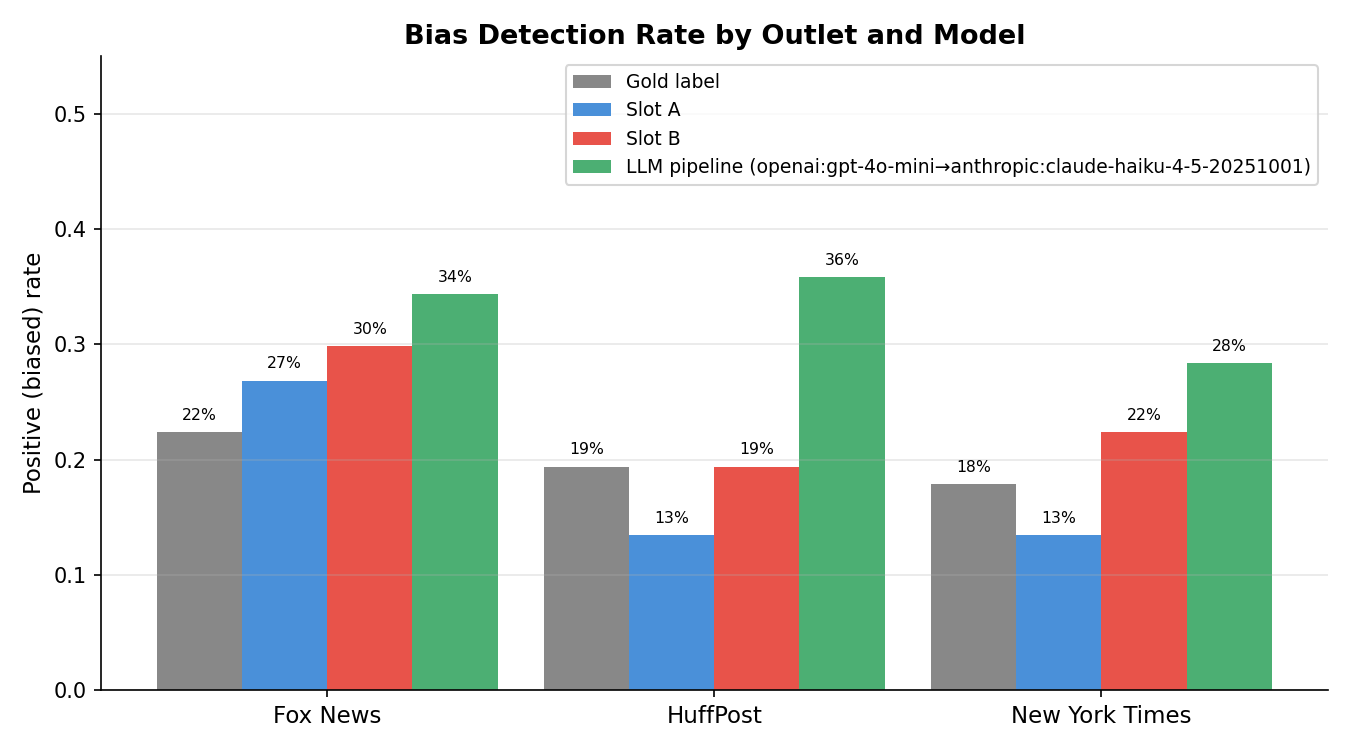
\includegraphics[width=0.7\textwidth]{viz_bias_rates_by_outlet.png}
\caption{Predicted bias rates by outlet across configurations.}
\label{fig:outlet}
\end{figure}

\begin{figure}[H]
\centering
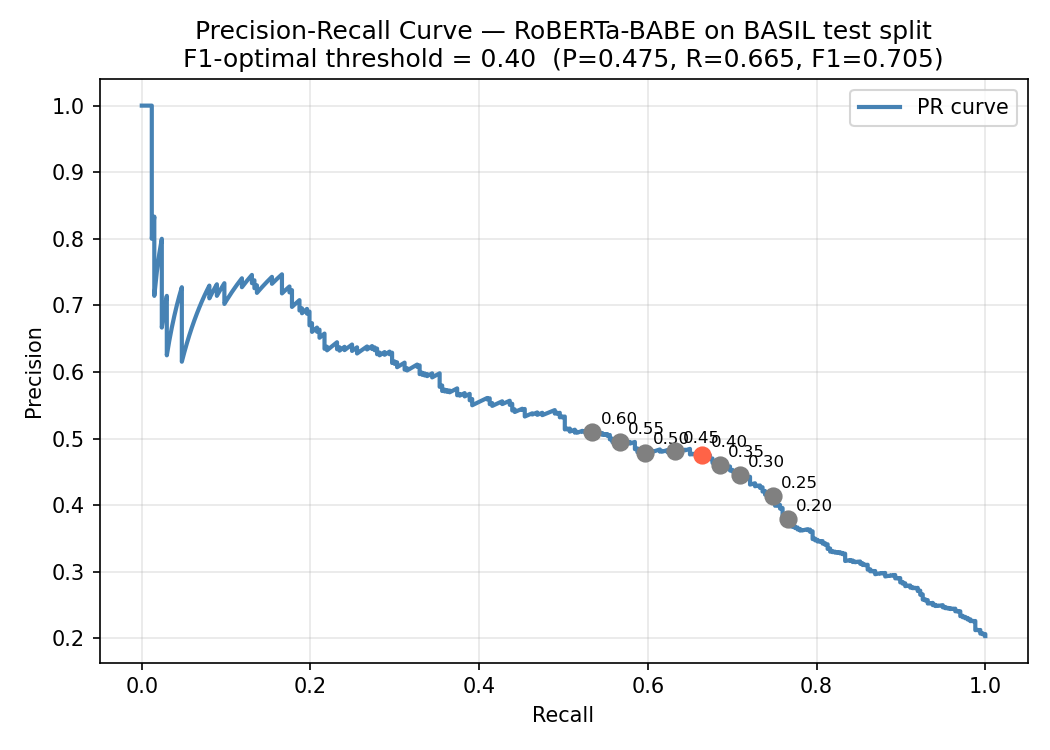
\includegraphics[width=0.55\textwidth]{precision_recall_curve.png}
\caption{Precision--recall curve from the threshold sweep. F1 is maximized at threshold 0.40.}
\label{fig:pr}
\end{figure}

\section{Analysis}

Three findings emerge from our results.

\paragraph{Finding 1: Zero-shot frontier LLMs are surprisingly competitive.}
The GPT$\rightarrow$Claude pipeline with BASIL-aligned prompts achieves a biased-class F1 of 0.472 and macro F1 of 0.641, compared to fine-tuned RoBERTa at 0.582 and 0.705 respectively --- gaps of 0.110 and 0.064 points. The comparison is intentionally asymmetric: RoBERTa was optimized directly on BASIL labels across 3 training epochs, while both LLMs receive only a structured prompt. This result suggests frontier LLMs have strong latent capacity for bias detection that approaches supervised baselines without any domain adaptation.

\paragraph{Finding 2: Definitional alignment between agents is critical.}
With naive prompts, the dual-agent pipeline achieved only macro F1{=}0.606 because the verifier applied a stricter definition of bias than BASIL uses --- systematically downgrading sentences where loaded language appeared in quoted speech, which BASIL labels as biased. This caused the verifier to remove true positives at a higher rate than false positives. Once both agents were given explicit BASIL definitions and few-shot examples, the verifier flipped from a liability to an asset: pipeline macro F1 rose from 0.606 to 0.641, the aligned pipeline also exceeds the auditor alone on biased-class F1 (0.472 vs.\ 0.462), and per-outlet macro F1 improves across all three outlets --- Fox ($+$0.017), HPO ($+$0.026), and NYT ($+$0.079). The lesson is architectural: in multi-agent systems, both agents must share the same evaluation criteria, or the second agent will work against the first.

\paragraph{Finding 3: Prompt engineering closes the gap more than expected.}
The full prompt engineering intervention --- BASIL definitions, few-shot examples, temperature{=}0 --- improved biased-class F1 by $+$0.125 (0.347$\rightarrow$0.472, Table~\ref{tab:ablation}), changed the sign of the verifier's contribution, and more than doubled recall from 0.300 to 0.625. The macro F1 gap versus RoBERTa narrowed from $-$0.099 (naive pipeline) to $-$0.064 (aligned pipeline). Both improvements were achieved with prompting alone, not fine-tuning. Further gains are likely available with stronger auditor models (GPT-4o, Claude Sonnet) or few-shot examples drawn directly from BASIL's held-out split.

Inter-model agreement ($\kappa{=}0.611$) remains substantively meaningful and is independent of the prompt changes, confirming that LLM-based bias judgments are reproducible across vendors. Fox content shows the largest inter-model disagreement (82.1\% agreement), consistent with politically charged framing being harder to classify consistently across providers with different training distributions.

\section{Conclusions}

\paragraph{Strengths.}
The architecture is modular and vendor-agnostic: any compliant LLM fills either slot via the MCP orchestration layer. Every model interaction is fully traceable through the SQLite audit log. With aligned prompts, the verifier demonstrably improves over the auditor alone, validating the dual-agent design. The live demo supports all four pipeline configurations in real time.

\paragraph{Weaknesses.}
Pipeline macro F1 (0.641) still trails the fine-tuned RoBERTa baseline (0.705). The LLM evaluation set is small (201 sentences) due to API cost. The auditor with aligned prompts over-flags aggressively (positive rate 44.8\% vs.\ gold rate $\approx$20\%), achieving high recall (0.750) at the cost of precision (0.333); the verifier partially corrects this by downgrading 24 of the 90 flagged sentences.

\paragraph{Limitations.}
BASIL is older, English-only, U.S. political news, and sentence-level labels miss higher-order framing effects. The threshold (0.40) was calibrated on RoBERTa's score distribution, not GPT's, which contributes to the auditor's over-flagging. Inference cost scales linearly with article length.

\paragraph{Future Work.}
(1) Calibrate the threshold directly on LLM score distributions rather than carrying over from RoBERTa; (2) test stronger auditor variants (GPT-4o, Claude Sonnet) to characterize the cost--quality frontier; (3) extend to document-level framing signals; (4) validate on newer corpora for generalization beyond 2010-era U.S. political reporting.

\section{Workflow}

Across Milestone 3, the project progressed from model setup and baseline construction to full pipeline evaluation, iterative prompt refinement, and a deployed demo. We began by selecting models, fixing the deprecated Claude endpoint issue, and fine-tuning RoBERTa on BASIL. We then ran the multi-provider and dual-agent experiments to produce the headline metrics and visualizations. After identifying that the verifier was hurting F1 due to a definition mismatch, we undertook prompt engineering (BASIL definitions, few-shot examples, temperature{=}0) to align both agents, improving pipeline macro F1 from 0.606 to 0.641 and biased-class F1 from 0.347 to 0.472, validating the dual-agent architecture. Finally we shipped a Flask backend integrated with the MCP layer and a React frontend, with final-week UI polish and cleanup.

\paragraph{Contributions.}
\begin{itemize}
\itemsep0pt
\item \textbf{Ryan Bi} --- core experiment and evaluation pipeline, all scripting (\texttt{run\_llm\_pipeline.py}, \texttt{run\_multi\_provider.py}, \texttt{visualize\_results.py}, \texttt{export\_audit\_log.py}), prompt engineering and iterative refinement, threshold sweep, metrics generation, the Flask demo server, and frontend--backend integration.
\item \textbf{Maheen Rassell} --- refactored the MCP server into a model-agnostic slot architecture (\texttt{bias\_surface.py}, \texttt{pipeline\_jobs.py}, \texttt{providers/}, \texttt{auditing/}) so providers are interchangeable via configuration rather than code changes.
\item \textbf{Terry Han} --- built the Vite/React frontend (App, styles, pipeline configuration UI, baseline comparison view) including the four-mode pipeline selector and the annotated-text bias view.
\end{itemize}

\paragraph{Repository.} \url{https://github.com/mrassell/dual-agent-bias-detection}

\end{document}
